\chapter{Modelos específicos de conductores}
\label{ch:specific-models}

En los capítulos anteriores se han decidido los modelos candidatos que conformarán el modelo de comportamiento de conductor general. Ahora que sabemos cuáles son las técnicas y arquitecturas que mejor se adecúan a este problema con los datos que disponemos, pasaremos a probarlas con los datos de los conductores específicos comprobando si:

\begin{itemize}
	\item Los errores y precisiones se mantienen en el orden del modelo global.
	\item Los modelos capturan las particularidades de cada sujeto de estudio.
\end{itemize}

Para ello, se comparará primero el modelo longitudinal global con los modelos entrenados de los sujetos. Posteriormente, se compararán los modelos de los sujetos contra los conjuntos de test de cada uno de ellos.

\section{Modelo longitudinal}

La arquitectura que se ha entrenado para cada uno de los sujetos ha sido la $MLP_2$. En la Figura~\ref{fig:lm-specific-training-validation-and-test-comparison} se muestra la evolución del \Acrshort{rmse}\index{RMSE} en test para cada uno de los sujetos tras entrenar los modelos con los parámetros indicado en el anterior capítulo.

\begin{figure}
	\centering
	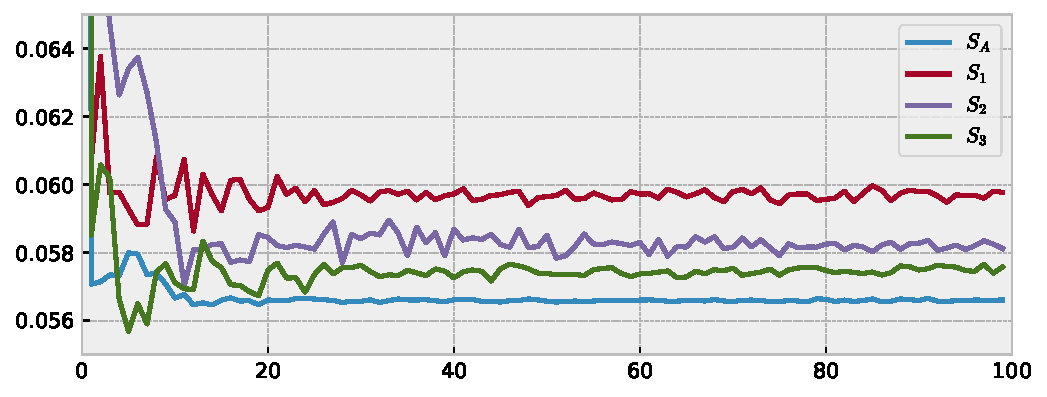
\includegraphics[width=\textwidth]{lm-specific-rmse-all-test-detail}
	\caption[Comparativa de la evolución del \gls{rmse} en test para los sujetos de la arquitectura seleccionada para el modelo longitudinal]{Comparativa de la evolución del error de test entre los sujetos de la arquitectura seleccionada para el modelo longitudinal. El \gls{rmse} en test en el caso del sujeto $S_2$ es muy alto (mayor que $0.2$) comparado con el error en el resto de sujetos y en el global.}
	\label{fig:lm-specific-training-validation-and-test-comparison}
\end{figure}

Se puede observar que el error en test de los sujetos es ligeramente mayor que el del conjunto global. Esto se puede explicar por la mayor capacidad de generalización de $S_A$ al haber sido entrenado con un conjunto de datos mayor. Los errores se resumen en la Tabla~\ref{tbl:lm-specific-rmse}.

\begin{table}
	\centering
	\caption[Resumen de los valores de \Acrshort{rmse} para los modelos específicos de comportamiento longitudinal]{Resumen de los valores de \Acrshort{rmse} para los modelos específicos de comportamiento longitudinal.}
	\label{tbl:lm-specific-rmse}
	\begin{tabularx}{\linewidth}{YYYYYY}
		\toprule
		\multirow{2}{*}{} & \multicolumn{3}{c}{\ac{rmse}}      \\ 
		& Entrenamiento & Validación & Test \\
		\midrule
		\rowcolor{black!20} $S_A$ & $0.056$ & $0.062$ & $0.057$  \\
		$S_1$ & $0.045$ & $0.039$ & $0.060$  \\
		\rowcolor{black!20} $S_2$ & $0.048$ & $0.047$ & $0.058$  \\
		$S_3$ & $0.055$ & $0.054$ & $0.058$  \\
		\bottomrule
	\end{tabularx}
\end{table}

\section{Control lateral}

En el caso del modelo del control lateral\index{lane-change}, la arquitectura con la que se han entrenado los modelos específicos es al $CNN_1$ (topología $c16$-$4$-$18$-$v$, $d128$). En la Figura~\ref{fig:lc-specific-rmse-all-test-detail} se muestra la evolución del \Acrshort{rmse}\index{RMSE} en test para cada uno de los sujetos tras entrenar los modelos con los parámetros indicado en el anterior capítulo.

\begin{figure}
	\centering
	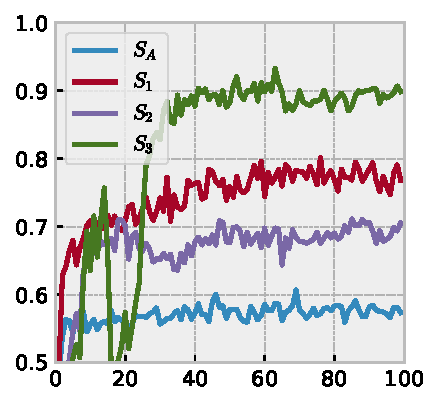
\includegraphics[width=\textwidth]{lc-specific-rmse-all-test-detail}
	\caption[\gls{rmse} en test entre los sujetos de la arquitectura seleccionada para el modelo de cambio de carril]{Comparativa de la evolución de la precisión en test entre los sujetos de la arquitectura seleccionada para el modelo de cambio de carril.}
	\label{fig:lc-specific-rmse-all-test-detail}
\end{figure}

La precisión alcanzada en los modelos específicos entrenados con esta arquitectura es mayor que la alcanzada por el modelo global. Tiene sentido ya que el modelo global se ha entrenado con el conjunto de datos global y por tanto no obedece exactamente al comportamiento de ningún perfil en concreto, mientras que en los modelos específicos sí. En la Tabla~\ref{tbl:lc-specific-accuracy} se exponen los valores de la precisión de este modelo.

\begin{table}
	\centering
	\caption[Precisión alcanzada para los modelos específicos de cambio de carril]{Resumen de los valores de precisión para los modelos específicos de cambio de carril.}
	\label{tbl:lc-specific-accuracy}
	\begin{tabularx}{\linewidth}{YYYYYY}
		\toprule
		\multirow{2}{*}{} & \multicolumn{3}{c}{\ac{rmse}}      \\ 
		& Entrenamiento & Validación & Test \\
		\midrule
		\rowcolor{black!20} $S_A$ & $0.588$ & $0.576$ & $0.573$  \\
		$S_1$ & $0.805$ & $0.763$ & $0.768$  \\
		\rowcolor{black!20} $S_2$ & $0.683$ & $0.708$ & $0.706$  \\
		$S_3$ & $0.727$ & $0.706$ & $0.710$  \\
		\bottomrule
	\end{tabularx}
\end{table}


\section{Personalización en modelos de conducción específicos}

Las anteriores secciones han mostrado cómo las topologías seleccionadas en los capítulos \nameref{ch:longitudinal-model} y \nameref{ch:lane-change-model} son adecuadas para modelar los comportamientos específicos de cada conductor, además del conjunto global.

Lo interesante es comprobar si estas topologías son capaces de capturar las diferencias entre conductores. Para ello, comprobaremos cómo se comportan cada uno de los conductores en todos los conjuntos de test.

En el caso del modelo longitudinal, el \ac{rmse} de cada uno de los conductores se mantiene más bajo que el del resto de los sujetos en su propio conjunto de test. En la Figura~\ref{fig:lm-subjects-comparison} se muestra gráficamente el perfil de aceleración de cada uno de los conductores sobre cada uno de los perfiles reales.

\begin{figure}
	\centering
	\subfloat[Sujeto $S_1$]{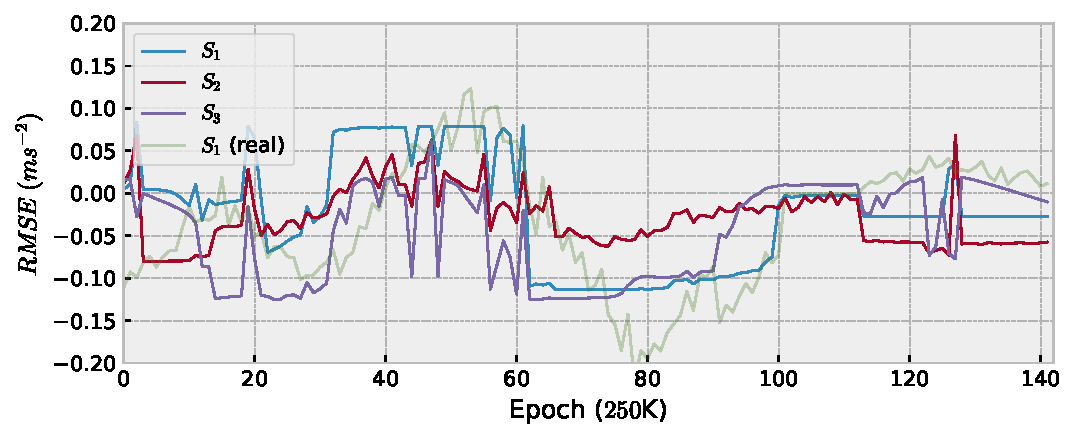
\includegraphics[width=\textwidth]{lm-subjects-comparison-with-edgar-acceleration-profiles}}\qquad
	\subfloat[Sujeto $S_2$]{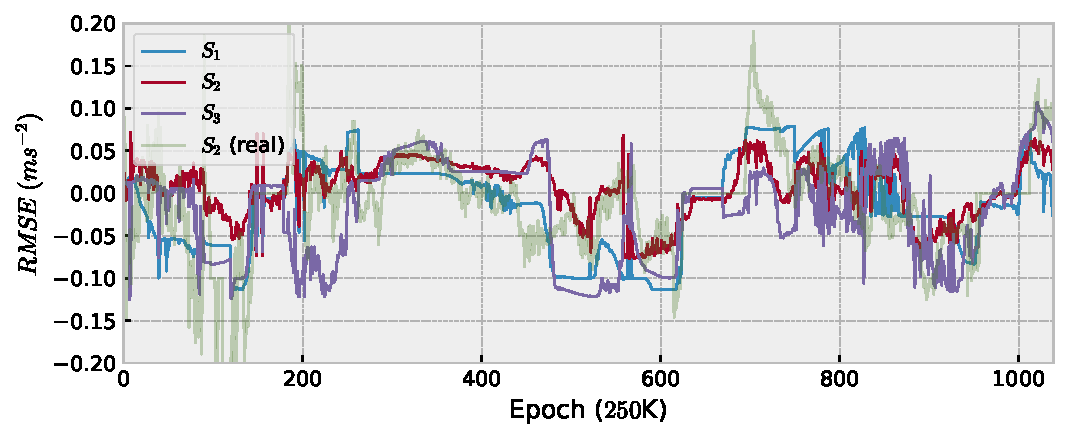
\includegraphics[width=\textwidth]{lm-subjects-comparison-with-jj-acceleration-profiles}}\qquad
	\subfloat[Sujeto $S_3$]{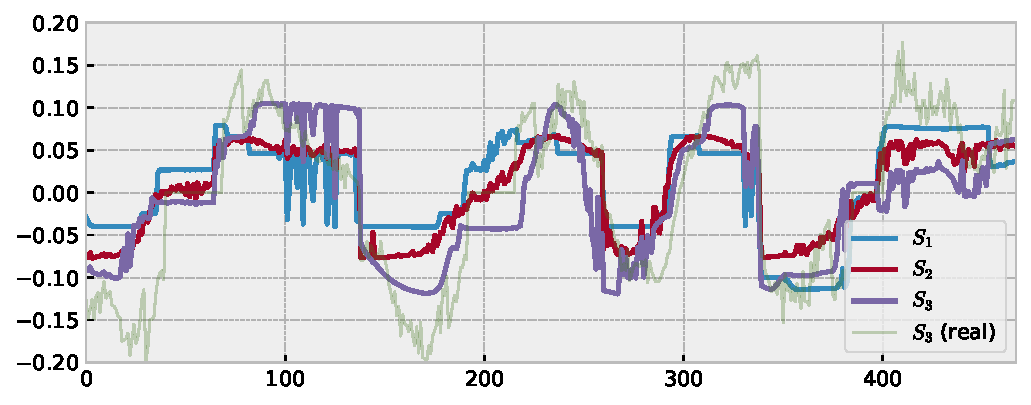
\includegraphics[width=\textwidth]{lm-subjects-comparison-with-miguel-acceleration-profiles}}
	\caption[Diferencia entre los perfiles de aceleración para los diferentes sujetos]{Perfiles de aceleración de los diferentes sujetos sobre el resto. Se puede observar que de todos ellos, los perfiles de los sujetos originales se aproximan más a sus respectivos perfiles que los del resto.}
	\label{fig:lm-subjects-comparison}
\end{figure}

Los valores de error cruzados entre sujetos se resumen en la tabla~\ref{tbl:lm-subjects-comparison}.

\begin{table}
	\centering
	\caption[Comparación de los errores de aceleración en los diferentes modelos longitudinales]{Comparación de los errores de aceleración en los diferentes modelos longitudinales. Las filas se corresponden con los recorridos mientras que las columnas se corresponden con los modelos que se han intentado ajustar a ellas.}
	\label{tbl:lm-subjects-comparison}
	\begin{tabularx}{\linewidth}{YYYY}
		\toprule
		& $S_1$ & $S_2$ & $S_3$ \\
		\midrule
		\rowcolor{black!20} $S_1$ & $0.059$        & $0.074$        & $0.070$ \\
		$S_2$ & $0.064$        & $0.058$        & $0.067$ \\
		\rowcolor{black!20} $S_3$ & $0.065$        & $0.065$        & $0.057$ \\
		\bottomrule
	\end{tabularx}
\end{table}

En el caso del modelo de cambio de carril\index{lane-change}, la comparativa la deberíamos hacer con respecto a las tasas de acierto en sus respectivos conjuntos de test. La Tabla~\ref{tbl:lc-subjects-comparison} muestra los índices de precisión de los sujetos sobre cada uno de los conjuntos de test de los demás.

\begin{table}
	\centering
	\caption[Comparación de la precisión para los diferentes modelos de cambio de carril]{Comparación de la precisión para los diferentes modelos de cambio de carril. Las filas se corresponden con los recorridos mientras que las columnas se corresponden con los modelos que se han intentado ajustar a ellas.}
	\label{tbl:lc-subjects-comparison}
	\begin{tabularx}{\linewidth}{YYYY}
		\toprule
		& $S_1$ & $S_2$ & $S_3$ \\
		\midrule
		\rowcolor{black!20} $S_1$ & $0.768$ & $0.314$ & $0.601$ \\
		$S_2$ & $0.601$ & $0.706$ & $0.511$ \\
		\rowcolor{black!20} $S_3$ & $0.648$ & $0.666$ & $0.710$ \\
		\bottomrule
	\end{tabularx}
\end{table}